\chapter{System Design}

System design is the process of defining the \cite {hocking2022unity} architecture, components, modules, interfaces, and data for a software system to meet specified requirements.

System design involves defining the overall architecture, breaking down the system into components and modules. Architectural design establishes the high-level structure, relationships between components, and communication mechanisms within the system.

\section{Architecture Design}
\textbf{Architecture design} is an important phase in system development that defines the structure and organization of a system. It defines the overall framework that indicates how various components interact, ensuring that the system meets functional requirements and performs efficiently. The architecture serves as a blueprint, guiding developers throughout the implementation process and enabling scaling and maintenance.

\begin{itemize}
\item \textbf{Component Identification:} Defining the individual components that make up the system, such as modules, libraries, and services.
\item  \textbf{Interaction Patterns:} Specifying how these components communicate and collaborate, including protocols, data flow, and interfaces.
\item \textbf{Design Patterns:} Utilizing established design patterns to solve common problems in software architecture, promoting re-usability and clarity.
\item \textbf{Scalability and Performance:} Considering how the architecture will support future growth and maintain performance standards under varying loads.
\end{itemize}
\subsection{Architecture Design of Gaming System}

The architecture of a game plays a very important role in engaging in responsive experiences \cite{kleppmann2017designing}. Following are the architectural components typically found in the gaming system.

\begin{figure}[H]
	\centering
	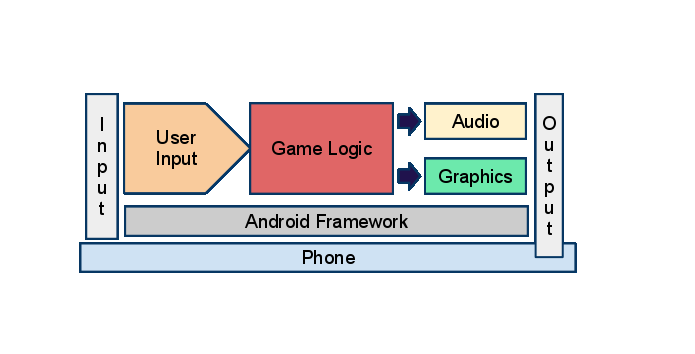
\includegraphics[width=18cm,height=12cm]{C://Users/PMLS/Desktop/Thesis/Latex Thesis/GameEngine.png}
	\caption{Architecture of a Gaming System}
	\label{fig:Architecture of Gaming System}
\end{figure}

\begin{itemize}
	\item\textbf{Game Engine:} A game's central component that handles input, handles physics, renders images, and coordinates game logic. With built-in tools and libraries, game engines such as Unity or Unreal Engine facilitate creation.
	\item \textbf{Game Client:} Players communicate with the game using this interface. It consists of the graphics systems, gaming mechanics, and user interface (UI). Input from the player is processed by the client, which also connects to the server and shows game statuses.
	\item \textbf{AI System:} This part controls how adversaries and NPCs (Non-Player Characters) behave, including how they respond to player input. Path finding, decision-making algorithms, and state machines are examples of AI.
	\item \textbf{Networking Module:}The networking module, which manages data exchange between clients and the game server, is crucial for multiplayer games. It guarantees the synchronization of player movements, game states, and other in-the-moment interactions.
	\item \textbf{Database/Storage System:}This component is responsible for storing the player data, player progress and other information that needs to be persisted in the database. A cloud-based database is a good option to be used depending on the game architecture.
	\item \textbf{Scripts:} Scripting capabilities offered by many games can be used to modify the game play depending on the game's architecture.
\end{itemize}

\subsection{Types of Architectures}
The following text discuss some of the Architecture that could be used in the game systems \cite{unity_architecture}.
\begin{itemize}
	\item \textbf{Modular Architecture: }A game with a modular architecture is easier to maintain and expand since it is divided into discrete modules for things like physics, AI, and rendered. Code reuse is encouraged by the separate development and testing of each module. Careful design is necessary to provide seamless integration and manage dependencies.
	\item \textbf{Entity-Component-System (ECS) Architecture: }Game logic is divided into entities (game objects), components (data), and systems (logic) in ECS design. This method encourages code reuse and the division of responsibilities while improving flexibility and efficiency. ECS scales well and works well for applications that require high performance, despite its initial complexity of implementation.
	\item \textbf{Client-Server Architecture: }With client-server architecture, user input and rendering are handled by the client, and game logic is executed on a server. Updates and management of multiplayer games are made easier by this centralization. But it needs stable network connections, and a strong infrastructure is needed because the server can become a bottleneck.
\end{itemize}

\subsection{Architecture of Proximity Assault}
To maximize its design and performance, the Proximity Assault Game makes use of both Entity-Component-System (ECS) architecture and modular architecture. The game's modular architecture separates the game's components (physics, AI, and rendering) to enable separate development and upkeep. By breaking down game objects into entities, components, and systems, ECS Architecture improves flexibility and efficiency while making game behaviors easier to handle and encouraging code reuse. This combination guarantees a game structure that is performant, scalable, and maintainable.

\subsubitem{Detailed Description of the Architecture}
\begin{enumerate}
	\item \textbf{Game Engine: Unity}
	\begin{itemize}
		\item Unity is the game engine used, providing tools for rendering, physics, and scripting.
	\end{itemize}
	
	\item \textbf{Core Systems}
	\begin{itemize}
		\item \textbf{Game Loop}: Manages the main cycle of the game, including updating game states, handling user inputs, and rendering frames.
		\item \textbf{Input Handling}: Captures and processes player inputs from devices like keyboards, mice, or game controllers.
		\item \textbf{Physics Engine}: Simulates realistic physics, including collision detection and response.
	\end{itemize}
	
	\item \textbf{Graphics and Rendering}
	\begin{itemize}
		\item \textbf{3D Models and Textures}: High-quality models and textures for characters, weapons, and environments.
		\item \textbf{Shaders}: Used to create realistic lighting and effects.
		\item \textbf{Animation System}: Manages character animations, including movement, shooting, and reloading.
	\end{itemize}
	
	\item \textbf{AI and NPCs}
	\begin{itemize}
		\item \textbf{AI System}: Controls the behavior of enemy NPCs, making them react intelligently to player actions.
		\item \textbf{Pathfinding}: Algorithms like A* for navigating the game environment.
	\end{itemize}
	
	\item \textbf{Audio}
	\begin{itemize}
		\item \textbf{Sound Effects}: Realistic gunfire, explosions, and ambient sounds.
		\item \textbf{Music}: Background music that enhances the gameplay experience.
		\item \textbf{Audio Engine}: Manages sound playback and spatial audio effects.
	\end{itemize}
	
	\item \textbf{User Interface (UI)}
	\begin{itemize}
		\item \textbf{HUD}: Displays health, ammo, mission objectives, and other critical information.
		\item \textbf{Menus}: Main menu, settings, and pause menu interfaces.
	\end{itemize}
	
	\item \textbf{Game Logic}
	\begin{itemize}
		\item \textbf{Mission System}: Defines and manages the objectives and progression of missions.
		\item \textbf{Weapon System}: Manages different weapons, their stats, and behaviors.
		\item \textbf{Health and Damage System}: Tracks player and enemy health, and calculates damage from attacks.
	\end{itemize}
	
	\item \textbf{Optimization}
	\begin{itemize}
		\item \textbf{Level of Detail (LOD)}: Reduces the complexity of distant objects to improve performance.
		\item \textbf{Occlusion Culling}: Prevents rendering of objects not visible to the player.
		\item \textbf{Performance Profiling}: Tools to monitor and optimize game performance.
	\end{itemize}
	
	\item \textbf{Development Tools}
	\begin{itemize}
		\item \textbf{Version Control}: Systems like Git for managing code and assets.
		\item \textbf{Integrated Development Environment (IDE)}: Tools like Visual Studio for coding and debugging.
	\end{itemize}
\end{enumerate}

\subsection{Architecture Design Diagram}
Below is the attached architecture diagram for the Proximity Assault.
The top-level package, \textbf{Unity Engine}, contains several key components organized into packages:

\begin{itemize}
	\item \textbf{Core Systems} includes foundational elements like Game Loop, Input Handling and Physics Engine
	\item \textbf{Graphics and Rendering} focuses on visual aspects with 3D Models Shaders and Animation Systems
	\item \textbf{AI and NPCs} covers AI System and Path-finding algorithms
	\item \textbf{Audio} involves Sound Effects, Music and Audio Engine
	\item \textbf{User Interface (UI)} manages HUD and Menus
	\item \textbf{Game Logic} handles Mission System, Weapon System and Health and Damage System
	\item \textbf{Optimization} improves performance through	 Level of Detail (LOD), Occlusion Culling and	Performance Profiling
	\item \textbf{Development Tools} supports Version Control Integrated Development Environment (IDE)
\end{itemize}

\begin{figure}[H]
	\centering
	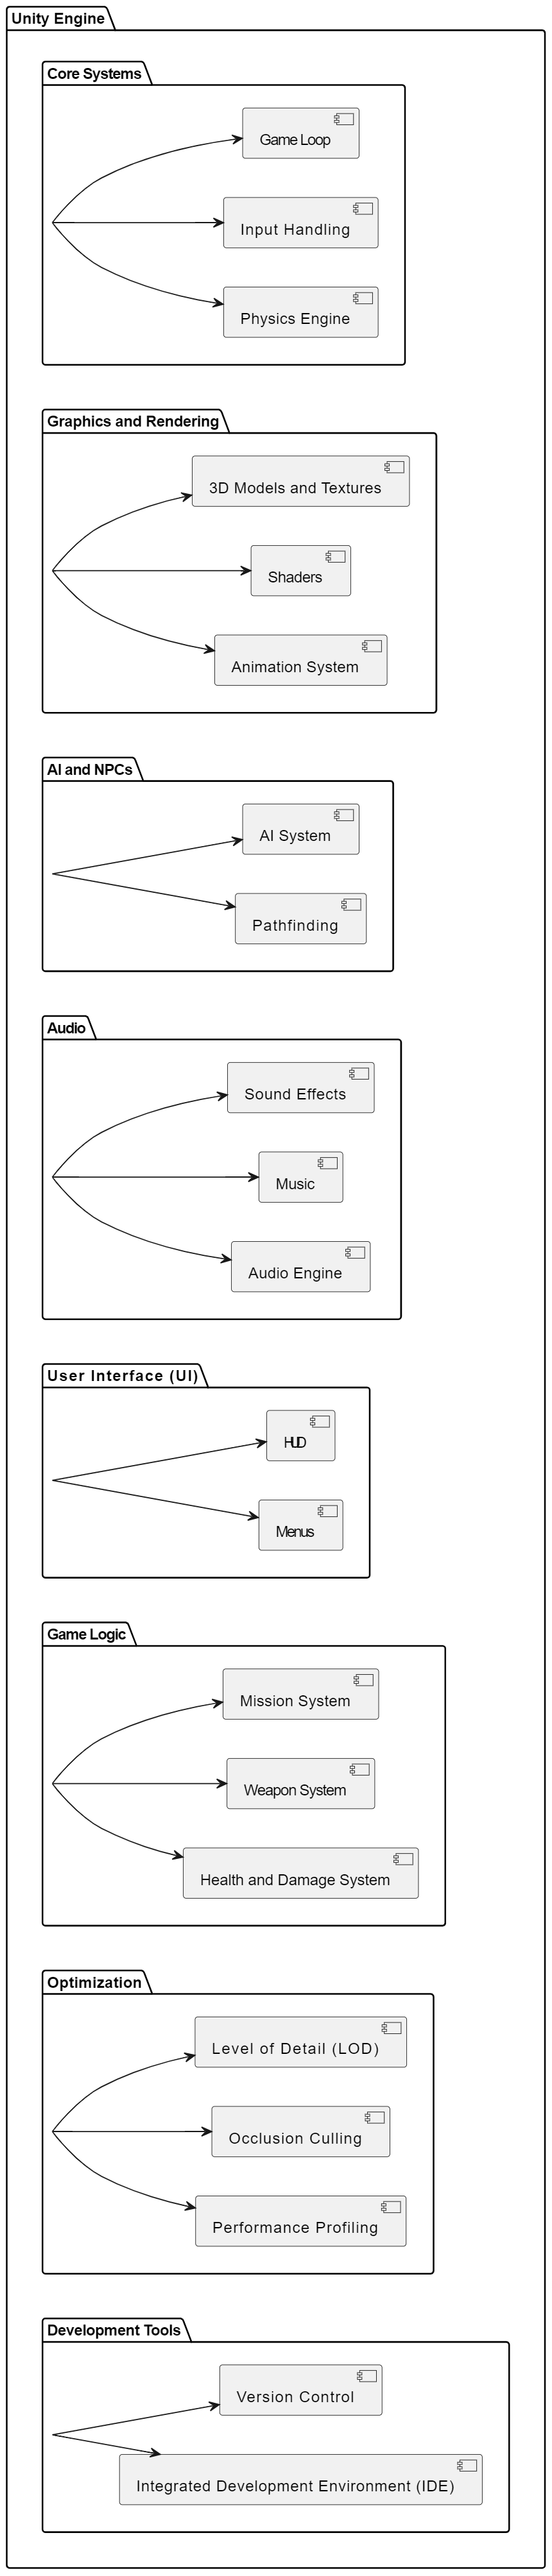
\includegraphics[width=4cm,height=12cm]{C://Users/PMLS/Desktop/Thesis/Latex Thesis/ArchitectureofProximityA4.png}
	\caption{Architecture Diagram}
	\label{fig:Architecture Design Diagram}
\end{figure}


\section{Component Level Design}
\begin{enumerate}
	\item \textbf{Core Systems}
	\begin{itemize}
		\item \textbf{Game Loop}
		\begin{itemize}
			\item \textbf{Update Cycle}: Handles periodic updates to game state and logic.
			\item \textbf{Render Cycle}: Manages rendering frames to the screen.
			\item \textbf{Event Handling}: Processes user input and system events.
		\end{itemize}
		\item \textbf{Input Handling}
		\begin{itemize}
			\item \textbf{Input Manager}: Captures and processes input from various devices (keyboard, mouse, game controllers).
			\item \textbf{Action Mapping}: Maps input actions to game functions (e.g., move, jump, shoot).
		\end{itemize}
		\item \textbf{Physics Engine}
		\begin{itemize}
			\item \textbf{Collision Detection}: Detects interactions between game objects.
			\item \textbf{Physics Simulation}: Simulates physical behaviors (e.g., gravity, momentum).
			\item \textbf{Rigid Body Dynamics}: Manages object movements and interactions based on physical properties.
		\end{itemize}
	\end{itemize}
	
	\item \textbf{Graphics and Rendering}
	\begin{itemize}
		\item \textbf{3D Models and Textures}
		\begin{itemize}
			\item \textbf{Model Loader}: Loads and processes 3D models from files.
			\item \textbf{Texture Mapping}: Applies textures to models.
		\end{itemize}
		\item \textbf{Shaders}
		\begin{itemize}
			\item \textbf{Vertex Shaders}: Handle vertex transformations and lighting.
			\item \textbf{Fragment Shaders}: Manage pixel-level coloring and effects.
		\end{itemize}
		\item \textbf{Animation System}
		\begin{itemize}
			\item \textbf{Animation Controller}: Manages animation states and transitions.
			\item \textbf{Bone System}: Handles skeletal animations for characters.
		\end{itemize}
	\end{itemize}
	
	\item \textbf{AI and NPCs}
	\begin{itemize}
		\item \textbf{AI System}
		\begin{itemize}
			\item \textbf{Behavior Trees}: Define complex NPC behaviors and decision-making processes.
			\item \textbf{Finite State Machines (FSM)}: Manage simple state-based behaviors.
		\end{itemize}
		\item \textbf{Pathfinding}
		\begin{itemize}
			\item \textbf{Navigation Mesh (NavMesh)}: Defines walkable areas in the game environment.
			\item \textbf{A* Algorithm}: Calculates optimal paths for NPC movement.
		\end{itemize}
	\end{itemize}
	
	\item \textbf{Audio}
	\begin{itemize}
		\item \textbf{Sound Effects}
		\begin{itemize}
			\item \textbf{Audio Clips}: Contains audio files for various game actions (e.g., gunfire, explosions).
			\item \textbf{Sound Manager}: Plays and manages sound effects.
		\end{itemize}
		\item \textbf{Audio Engine}
		\begin{itemize}
			\item \textbf{Spatial Audio}: Provides 3D audio effects based on player position.
			\item \textbf{Volume Control}: Adjusts the volume of different audio sources.
		\end{itemize}
	\end{itemize}
	\item \textbf{User Interface (UI)}
	\begin{itemize}
		\item \textbf{HUD (Heads-Up Display)}
		\begin{itemize}
			\item \textbf{Health Bar}: Displays the player's current health.
			\item \textbf{Mission Objectives}: Lists current goals and progress.
		\end{itemize}
		\item \textbf{Menus}
		\begin{itemize}
			\item \textbf{Main Menu}: Provides options for starting the game, loading saved games, and accessing settings.
			\item \textbf{Settings Menu}: Allows adjustments to game settings (e.g., audio, controls).
			\item \textbf{Pause Menu}: Provides options to resume, restart, or exit the game.
		\end{itemize}
	\end{itemize}
	
	\item \textbf{Game Logic}
	\begin{itemize}
		\item \textbf{Mission System}
		\begin{itemize}
			\item \textbf{Mission Manager}: Controls mission objectives, tracking, and progression.
		\end{itemize}
		\item \textbf{Weapon System}
		\begin{itemize}
			\item \textbf{Weapon Manager}: Handles weapon switching, equipping, and firing mechanics.
			\item \textbf{Weapon Stats}: Manages weapon attributes such as damage, range, and fire rate.
		\end{itemize}
		\item \textbf{Health and Damage System}
		\begin{itemize}
			\item \textbf{Health Manager}: Tracks health points for the player and NPCs.
			\item \textbf{Damage Calculation}: Calculates damage dealt to characters and applies effects.
		\end{itemize}
	\end{itemize}
	\item \textbf{Development Tools}
	\begin{itemize}
		\item \textbf{Version Control tools include Git and GitHub}
		\item \textbf{Visual Studio}
	\end{itemize}
\end{enumerate}

\begin{figure}[H]
	\centering
	
\includegraphics[width=6cm,height=16cm]{C://Users/PMLS/Desktop/Thesis/Latex Thesis/ComponentDesign.png}
	\caption{Component Diagram}
	\label{fig:Component Diagram}
\end{figure}


\section{Detailed Activity Diagram for a Game}

\begin{enumerate}
	\item \textbf{Player Starts the Game}
	
	\item \textbf{Main Menu}

	\item \textbf{New Game or Load Saved Game}
	
	\item \textbf{Main Game Loop}
	
	\item \textbf{Player Actions and Events}


	\item \textbf{Mission Complete}
	
	\item \textbf{Pause Menu}
	
	\item \textbf{Game Over}

\end{enumerate}
\section{Activity Diagram}
\begin{figure}[H]
	\centering
    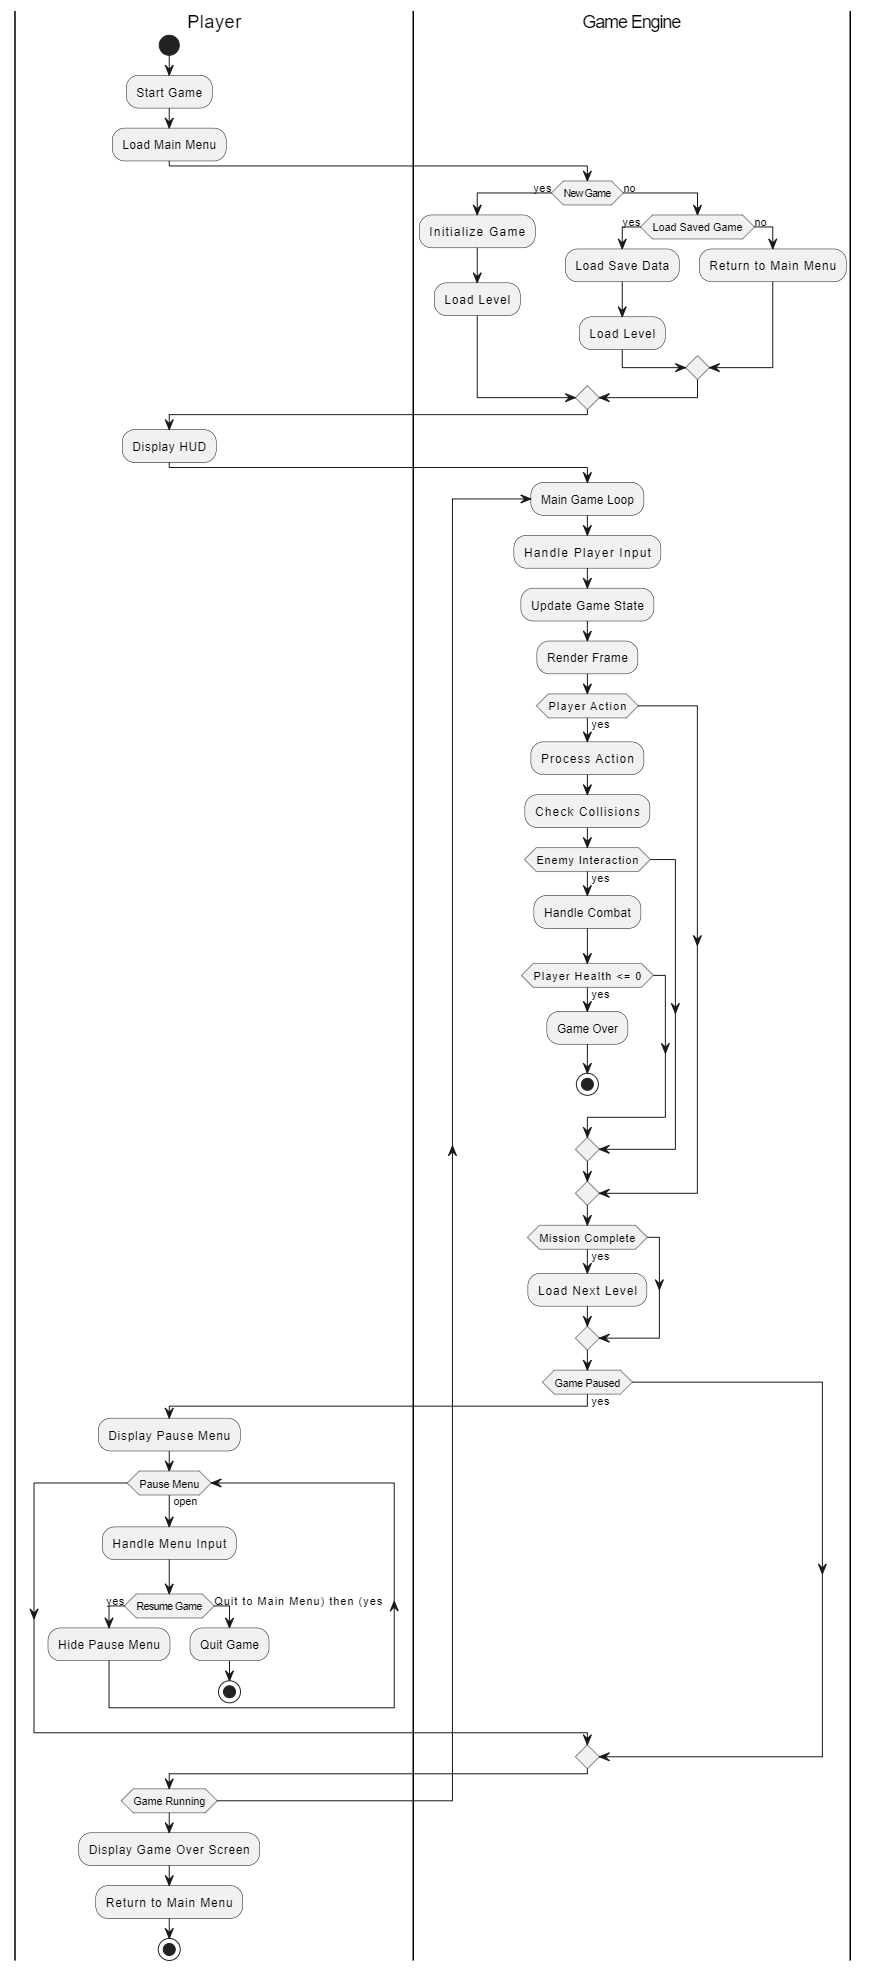
\includegraphics[width=12cm,height=16cm]{C://Users/PMLS/Desktop/Thesis/Latex Thesis/ActivityDiagram.png}
	\caption{Activity Diagram}
	\label{fig:Activity Diagram}
\end{figure}
\section{Class Diagram}
A class diagram for a gaming system typically includes classes such as \texttt{Game}, \texttt{Player}, \texttt{Enemy}, \texttt{Level}, \texttt{Weapon}, \texttt{Mission}, and various managers (e.g., \texttt{AudioManager}, \texttt{InputManager}, \texttt{PhysicsEngine}, \texttt{GraphicsEngine}, \texttt{AISystem}). These classes interact to represent the game's core components, manage gameplay elements, handle player inputs, simulate physics, render graphics, and control AI behaviors. Each class has specific attributes and methods that define their roles and responsibilities within the game.

\begin{itemize}
	\item \textbf{Game Class}: The main class containing the core components and systems.
	\item \textbf{Player and Enemy Classes}: Representing the player and enemies with attributes and methods for movement, attack, etc.
	\item \textbf{Level and Objective Classes}: Handling levels and their objectives.
	\item \textbf{Weapon, WeaponManager, and HUD Classes}: Managing weapons, HUD elements, and their updates.
	\item \textbf{Mission and MissionManager Classes}: Managing missions and their statuses.
	\item \textbf{AudioManager, MusicTrack, and SoundEffect Classes}: Handling audio playback.
	\item \textbf{InputManager Class}: Processing player inputs.
	\item \textbf{PhysicsEngine and GraphicsEngine Classes}: Simulating physics and rendering graphics.
	\item \textbf{AISystem, Behavior, and Pathfinding Classes}: Managing AI behaviors and pathfinding.
	\item \textbf{Vector3 Class}: Representing 3D vectors.
	\item \textbf{Enumerations}: Defining various game states, enemy types, behavior types, and actions.
\end{itemize}

\begin{figure}[H]
	\centering
	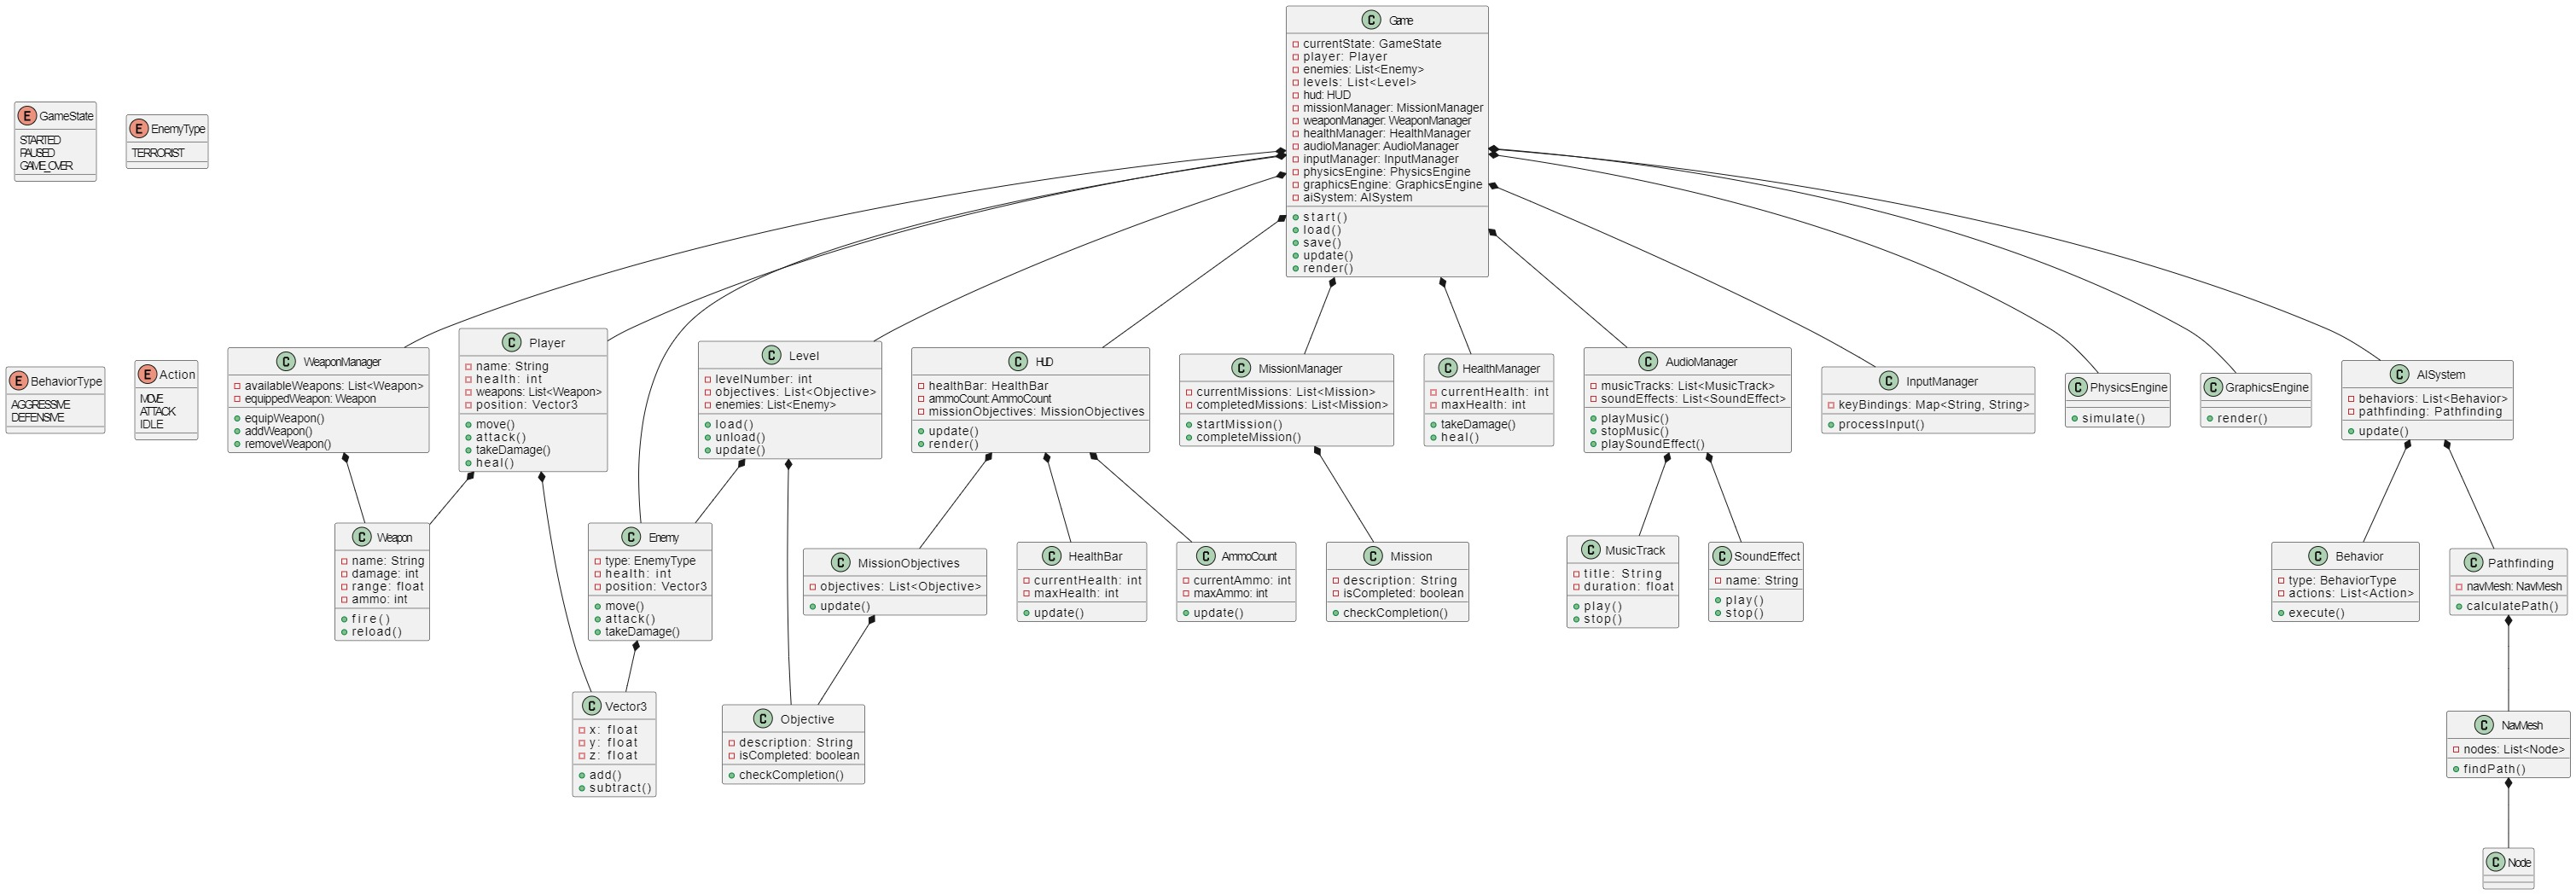
\includegraphics[width=16cm,height=6cm]{C://Users/PMLS/Desktop/Thesis/Latex Thesis/ClassDiagram.jpg}
	\caption{Class Diagram}
	\label{fig:Class Diagram}
\end{figure}


\section{Data Flow Diagram}
A class diagram for a gaming system typically includes classes such as \texttt{Game}, \texttt{Player}, \texttt{Enemy}, \texttt{Level}, \texttt{Weapon}, \texttt{Mission}, and various managers (e.g., \texttt{AudioManager}, \texttt{InputManager}, \texttt{PhysicsEngine}, \texttt{GraphicsEngine}, \texttt{AISystem}). These classes interact to represent the game's core components, manage gameplay elements, handle player inputs, simulate physics, render graphics, and control AI behaviors. Each class has specific attributes and methods that define their roles and responsibilities within the game.

\subsection{Level 0 Data Flow Diagram (DFD)}
A Level 0 Data Flow Diagram (DFD), also known as a context diagram, represents the entire system as a single process. It provides a high-level overview of the system's interactions with external entities such as users, other systems, or data sources. Here’s a simple explanation:

\begin{itemize}
	\item \textbf{Single Process}: The whole system is shown as one process, representing all the main functions and operations.
	\item \textbf{External Entities}: It includes all the external entities that interact with the system (e.g., users, other systems).
	\item \textbf{Data Flows}: Shows the flow of data between the system and these external entities.
	\item \textbf{High-Level View}: It’s a big-picture view that doesn't dive into the details of internal processes or data stores within the system.
\end{itemize}

A Level 0 DFD provides a basic, overall picture of how the system interacts with its environment.
\begin{figure}[H]
	\centering
	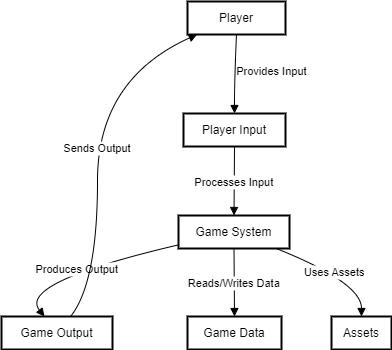
\includegraphics[width=10cm,height=6cm]{C://Users/PMLS/Desktop/Thesis/Latex Thesis/DataFlowDiagramLevel0ng.png}
	\caption{Level 0 DFD}
	\label{fig:Level 0 Data Flow Diagram}
\end{figure}


\subsubsection{Explaination}

\begin{itemize}
	\item \textbf{Player}: Provides input to the game system and receives game output.
	\item \textbf{Game System}: Processes player input, interacts with game data and assets, and produces game output.
	\item \textbf{Player Input}: Captures and processes input from the player.
	\item \textbf{Game Output}: The result of the game system processing, sent back to the player.
	\item \textbf{Game Data}: Stores and retrieves game-related data.
	\item \textbf{Assets}: Provides game assets like models, textures, and audio.
\end{itemize}

\subsection{Level 1 Data Flow Diagram (DFD)}
A Level 1 Data Flow Diagram (DFD) for an action shooting game represents a detailed view of the system. It breaks down the single process from the Level 0 DFD into several sub-processes and shows data flows between them.
\begin{itemize}
	\item \textbf{Player Input Handling}: Captures and processes inputs from the player, such as movement commands and shooting actions.
	\item \textbf{Game Logic}: Manages the core mechanics of the game, including player movements, shooting mechanics, collision detection, and health management.
	\item \textbf{AI System}: Manages the behavior of enemies, including their movements, attacks, and decision-making.
	\item \textbf{Rendering Engine}: Handles the visual output of the game, rendering the game world, characters, and effects based on the current game state.
	\item \textbf{Audio Engine}: Manages audio playback, including background music, sound effects, and voiceovers.
	\item \textbf{Game Data Management}: Stores and retrieves game-related data, such as player progress, scores, and game state.
\end{itemize}

The Level 1 DFD provides a detailed view of how the game system processes player inputs, manages game logic, handles enemy AI, and produces visual and audio outputs.

\begin{figure}[H]
	\centering
	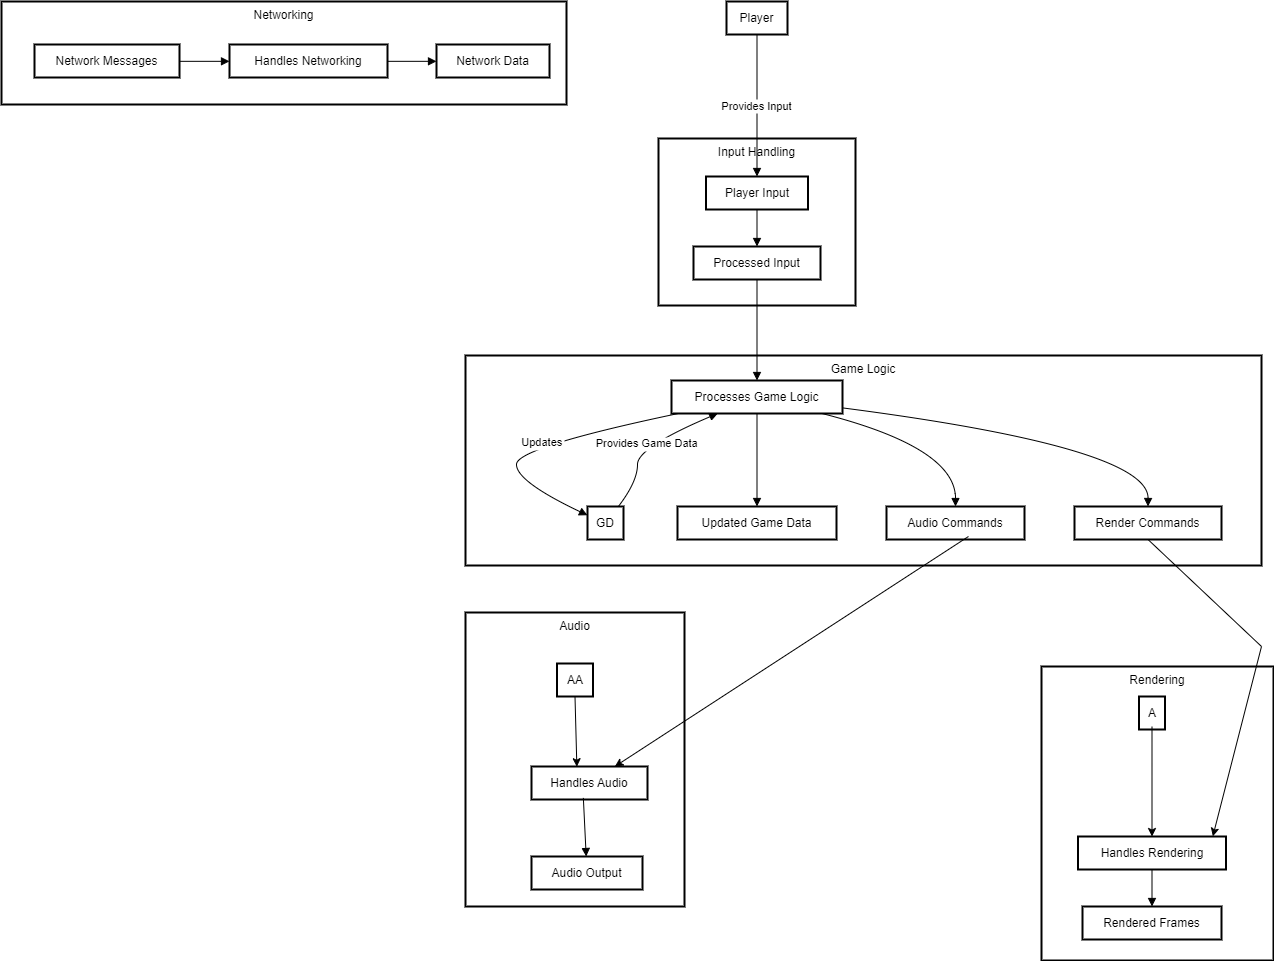
\includegraphics[width=16cm,height=8cm]{C://Users/PMLS/Desktop/Thesis/Latex Thesis/DataFlowDiagramLevel1.png}
	\caption{Level 1 DFD}
	\label{fig:Level 1 Data Flow Diagram}
\end{figure}


\subsubsection{Explaination}
\begin{itemize}
	\item \textbf{Player (P)}: Provides input to the system.
	\item \textbf{Input Handling (IH)}: Captures and processes player input.
	\item \textbf{Player Input (PI)}: Raw input from the player.
	\item \textbf{Processed Input (PIn)}: Input after processing, sent to Game Logic.
	\item \textbf{Game Logic (GL)}: Core logic of the game.
	\item \textbf{Processes Game Logic (GLP)}: Handles game mechanics and logic.
	\item \textbf{Game Data (GD)}: Stores game state data, both read and written by Game Logic.
	\item \textbf{Updated Game Data (UGD)}: Updated state of the game.
	\item \textbf{Render Commands (RC)}: Instructions for rendering the game visuals.
	\item \textbf{Audio Commands (AC)}: Instructions for game audio.
	\item \textbf{Rendering (R)}: Manages the visual output of the game.
	\item \textbf{Handles Rendering (RP)}: Renders frames using provided assets.
	\item \textbf{Rendered Frames (RF)}: Output frames to be displayed.
	\item \textbf{Assets (A)}: Visual assets like models and textures.
	\item \textbf{Audio (AU)}: Manages the audio output of the game.
	\item \textbf{Handles Audio (AP)}: Processes audio commands and assets.
	\item \textbf{Audio Output (AO)}: Output sound to be played.
	\item \textbf{Audio Assets (AA)}: Audio files and sound effects.
\end{itemize}
\subsubsection{Networking Component in DFD}
The Networking section in the Data Flow Diagram (DFD) is included as a placeholder for potential future development. While the current version of the game is designed for offline play.
\section{Data Design}
Data design involves structuring and organizing data to efficiently store, manage, and retrieve it within a system.
The data design diagram focuses on how the data is structured and managed.
\\
\begin{figure}[H]
	\centering
    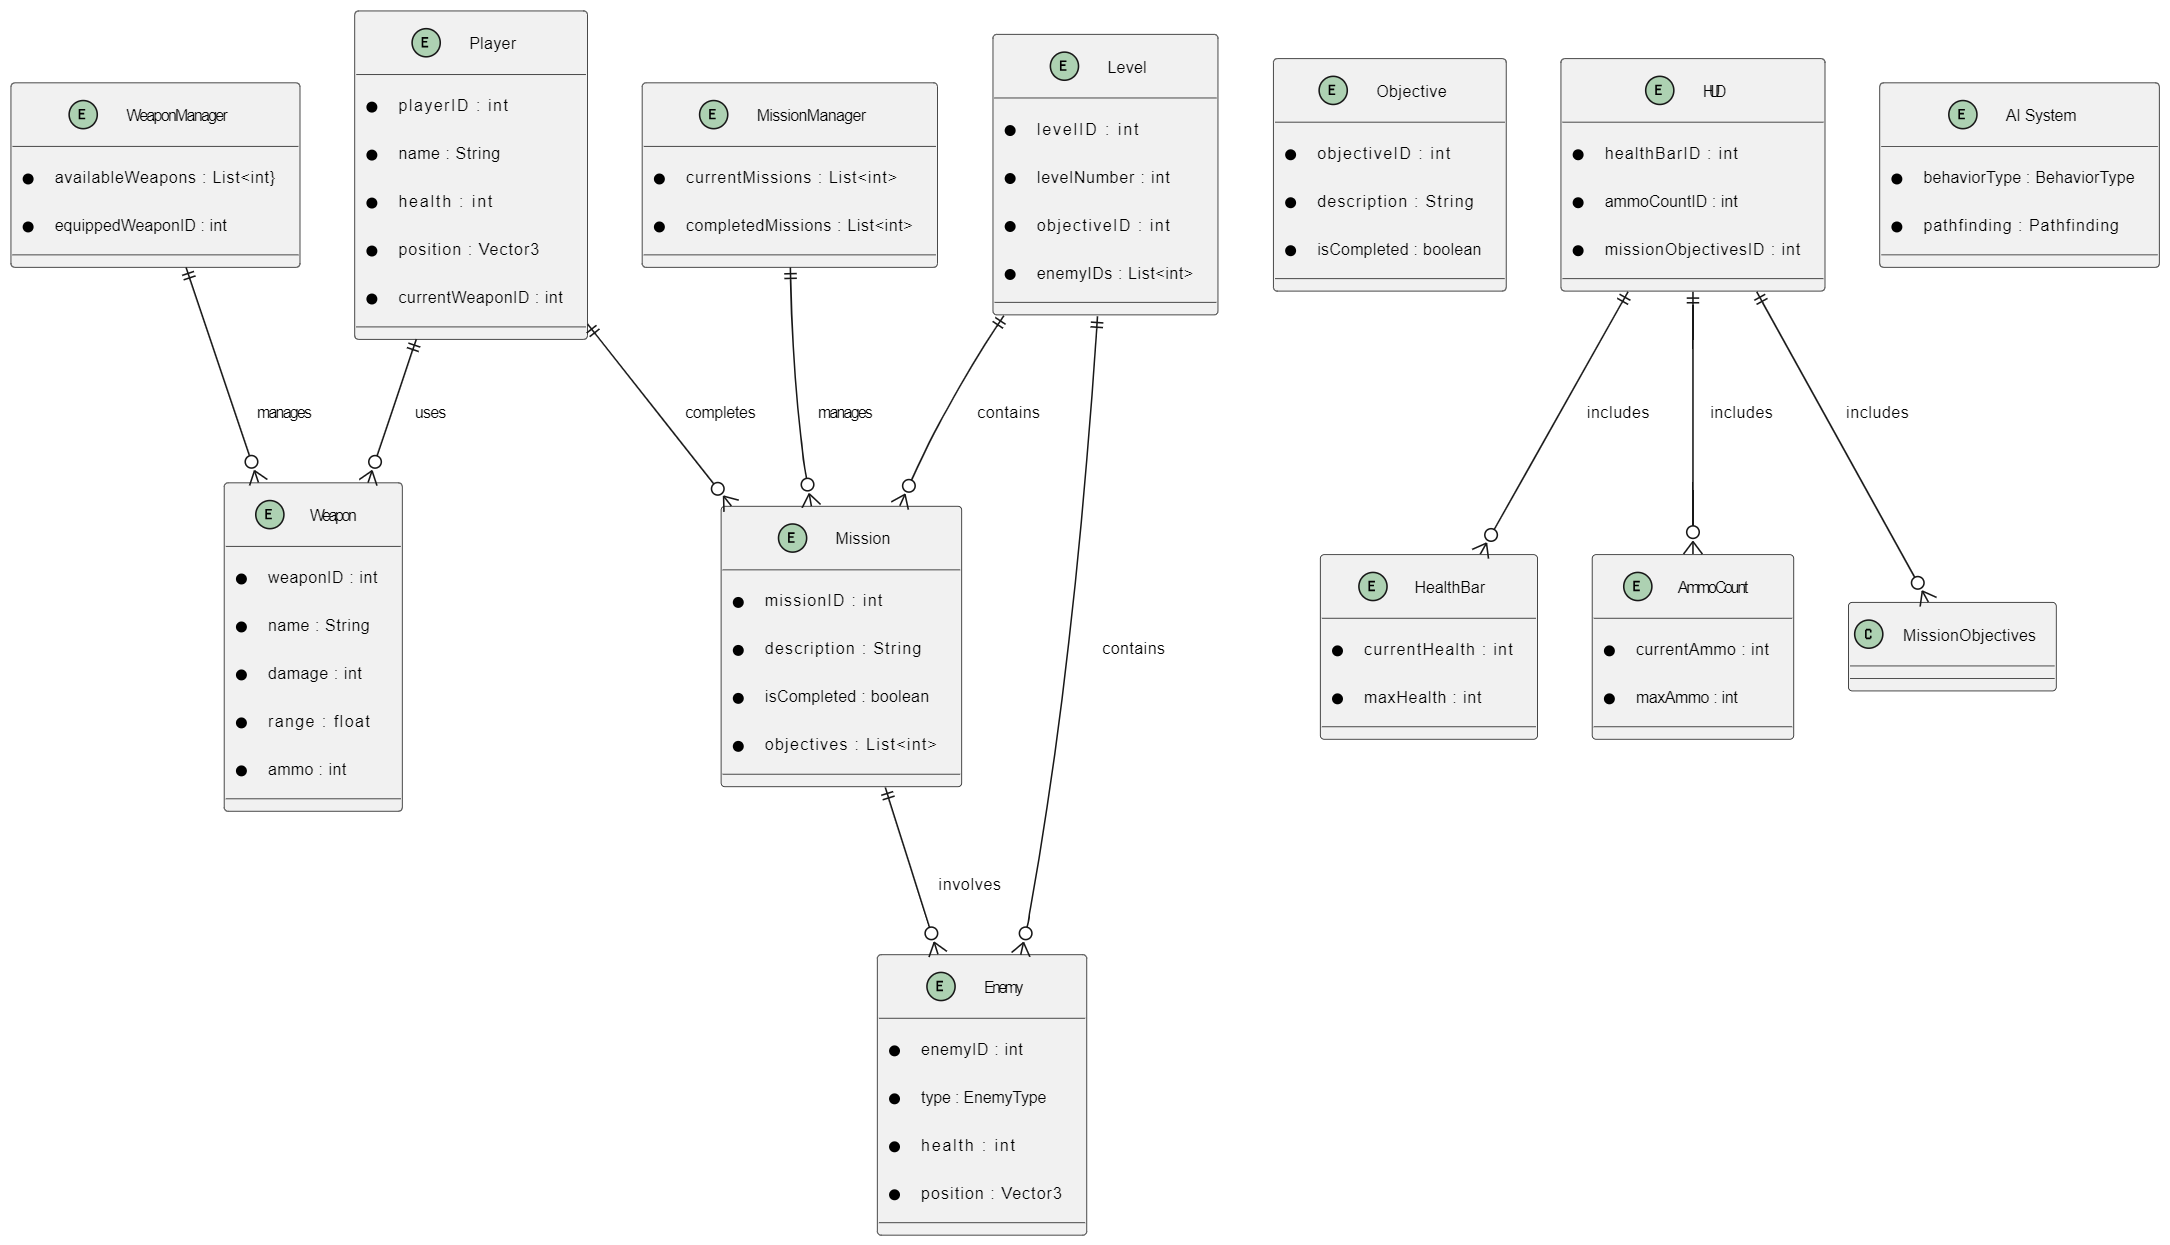
\includegraphics[width=14cm,height=10cm]{C://Users/PMLS/Desktop/Thesis/Latex Thesis/DataDesign.png}
	\caption{Data Design}
	\label{fig:Data Design Diagram}
\end{figure}

\subsection{Major Business Entities}
\textbf{Player:}
Represents the main character. This entity is central to the game, tracking important attributes like health, position, and equipped weapon.
\\
\\
\textbf{Weapon:}
Represents the tools player uses to attack enemies.
\\
\\
\textbf{Enemy:}
Represents the adversaries the player encounters. Enemies have attributes like type, health, and position, determining their behavior and how challenging they are for the player.
\\
\\
\textbf{Level:}
Represents the different stages or environments in the game. Each level contains objectives and enemies, and its structure impacts the game's progression.
\\
\\
\textbf{Objective:}
Represents specific goals the player must achieve within a level or mission.
\\
\\
\textbf{HUD (Heads-Up Display):}
Represents the on-screen display elements that provide the player with essential information like health, ammo, and mission status.
\\
\\
\textbf{HealthBar}
A component of the HUD that shows the player's current health.
\\
\\
\textbf{AmmoCount:}
Another component of the HUD that displays the current ammo count.
\\
\\
\textbf{AI System:}
Represents the system controlling enemy behavior and navigation.

\subsection{Entity Relationship Diagram}
The Entity-Relationship Diagram (ERD) for the game illustrates the main components and how they interact with each other.
\begin{figure}[H]
	\centering
	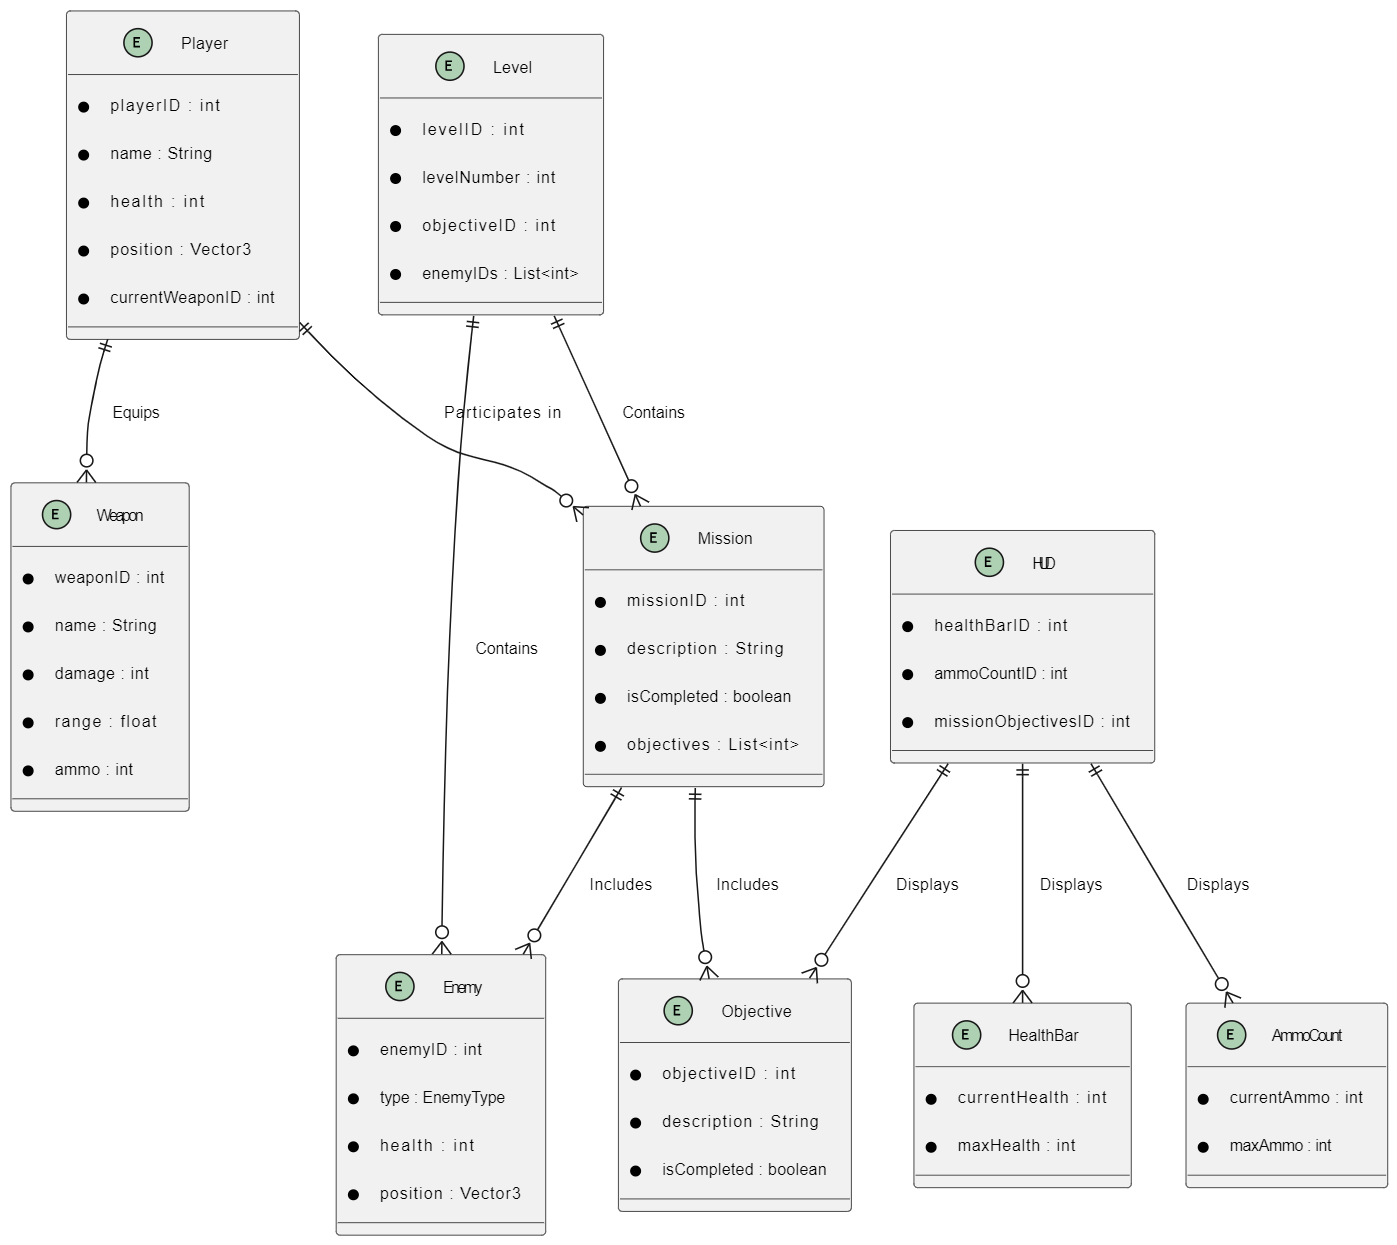
\includegraphics[width=16cm,height=10cm]{C://Users/PMLS/Desktop/Thesis/Latex Thesis/ERD (1).png}
	\caption{Entity Relationship Diagram}
	\label{fig:ERD}
\end{figure}
\subsubsection{Explanation:}

\textbf{Entities and Attributes:}

\begin{itemize}
	\item \textbf{Player}: Represents the player with attributes for ID, name, health, position, and currently equipped weapon.
	\item \textbf{Weapon}: Represents weapons with attributes for ID, name, damage, range, and ammo count.
	\item \textbf{Enemy}: Represents enemies with attributes for ID, type, health, and position.
	\item \textbf{Level}: Represents game levels with attributes for ID, level number, objectives, and list of enemies.
	\item \textbf{Objective}: Represents mission objectives with ID, description, and completion status.
	\item \textbf{Mission}: Represents missions with ID, description, completion status, and associated objectives.
	\item \textbf{HUD}: Represents the Heads-Up Display with IDs for health bar, ammo count, and mission objectives.
	\item \textbf{HealthBar and AmmoCount}: Display current and maximum health and ammo, respectively.
\end{itemize}

\textbf{Relationships:}

\begin{itemize}
	\item \textbf{Player - Weapon}: Players equip weapons.
	\item \textbf{Player - Mission}: Players participate in missions.
	\item \textbf{Mission - Objective}: Missions include objectives.
	\item \textbf{Level - Mission}: Levels contain missions.
	\item \textbf{Level - Enemy}: Levels contain enemies.
	\item \textbf{Mission - Enemy}: Missions involve enemies.
	\item \textbf{HUD - HealthBar}: HUD displays health bar information.
	\item \textbf{HUD - AmmoCount}: HUD displays ammo count information.
	\item \textbf{HUD - Objective}: HUD displays mission objectives.
\end{itemize}

\subsection{User-Interface Design}
\subsubsection{UI Design Decisions}
A minimalist approach was used to design the game UI and just implement the main features to make it functional. The color scheme of the game was set to be a light color so that it can be more adjusted to the user's eyes. The UI was completed implemented from the unity asset store while some of the rectifications were made using tools such as Figma or Adobe Packages for designing the interface.


